\let\negmedspace\undefined
\let\negthickspace\undefined
\documentclass[journal]{IEEEtran}
\usepackage[a5paper, margin=10mm, onecolumn]{geometry}
\usepackage{lmodern} % Ensure lmodern is loaded for pdflatex
\usepackage{tfrupee} % Include tfrupee package

\setlength{\headheight}{1cm} % Set the height of the header box
\setlength{\headsep}{0mm}     % Set the distance between the header box and the top of the text

\usepackage{gvv-book}
\usepackage{gvv}
\usepackage{cite}
\usepackage{amsmath,amssymb,amsfonts,amsthm}
\usepackage{algorithmic}
\usepackage{graphicx}
\usepackage{textcomp}
\usepackage{xcolor}
\usepackage{txfonts}
\usepackage{listings}
\usepackage{enumitem}
\usepackage{mathtools}
\usepackage{gensymb}
\usepackage{comment}
\usepackage[breaklinks=true]{hyperref}
\usepackage{tkz-euclide} 
\usepackage{listings}
\usepackage{gvv}                                        
\def\inputGnumericTable{}                                 
\usepackage[latin1]{inputenc}                                
\usepackage{color}                                            
\usepackage{array}                                            
\usepackage{longtable}                                       
\usepackage{calc}                                             
\usepackage{multirow}                                         
\usepackage{hhline}                                           
\usepackage{ifthen}                                           
\usepackage{lscape}
\usepackage{tikz}
\usepackage{tcolorbox}
\usetikzlibrary{matrix}
\usepackage{url}
\usepackage{xcolor}\begin{document}

\bibliographystyle{IEEEtran}
\vspace{3cm}

\title{10.3.3.1.4}
\author{EE24BTECH110021 - Eshan Ray}
% \maketitle
% \newpage
% \bigskip
{\let\newpage\relax\maketitle}
\textbf{Question:}
Solve the following system of equations,
\begin{align}
  0.2x + 0.3y &=1.3\\
  0.4x + 0.5y &= 2.3
\end{align}

\solution{\\
The following system of equations can be written in matrix form:-
\begin{align}
  Ax&= b  
\end{align}
where,
\begin{align}
    A &= \myvec{0.2&0.3\\0.4&0.5}\\
    b &= \myvec{1.3\\2.3}\\
    x &= \myvec{x\\y}\\
    \myvec{0.2&0.3\\0.4&0.5}\myvec{x\\y} &= \myvec{1.3\\2.3}
\end{align}
Using row reduction on augmented matrix $[A|b]$ we get,
\begin{align}
    \myvec{0.2 & 0.3 &| 1.3\\0.4 & 0.5&|2.3}
\end{align}
$R_2 \rightarrow R_2 - 2R_1$
\begin{align}
    \myvec{0.2 & 0.3 &|1.3\\ 0 & -0.1 &|-0.3}
\end{align}
$R_1\rightarrow R_1 + 3R_2$
\begin{align}
    \myvec{0.2 & 0 &|0.4\\0 & -0.1 &|-0.3}
\end{align}
$R_1\rightarrow \frac{R_1}{0.2} , R_2\rightarrow \frac{R_2}{-0.1}$
\begin{align}
    \myvec{1 &0 &|2\\0 & 1 &|3}
\end{align}
So, the point of intersection is $\brak{2,3}$
}\\
\textbf{Computational Solution}:
\textbf{LU Decomposition}\\
%Representing using matrices,
%\begin{align}
    %\myvec{
   %     2 & 1\\
  %      2 & -1
 %   } \myvec{x \\ y}= \myvec{ 6 \\ 2}
%\end{align}
Solving the system of equations matrix form $Ax=b$ by LU Decomposition where $A$ can be represented as a product of a lower triangular matrix $L$ and an upper triangular matrix $U$
\begin{align}
    A\vec{x} = LU\vec{x} = \vec{b}
\end{align}
Applying row reduction on $A$, we get,
\begin{align}
  \myvec{0.2&0.3\\0.4&0.5} \xrightarrow{R_2 = R_2 - 2R_1} \myvec{0.2&0.3\\0 & -0.1}
\end{align}
Let 
\begin{align}
    L = \myvec{1 & 0\\ l_{21} & 1}
\end{align}
$l_{21}$ is the multiplier used to zero $a_{21}$, so $l_{21} = 2$.\\
Now,
\begin{align}
    A = \myvec{0.2&0.3\\0.4&0.5} = \myvec{1 & 0 \\ 2 & 1}\myvec{0.2&0.3\\0&-0.1}
\end{align}
We have obtained LU Decomposition of the matrix $A$.\\
The LU Decomposition of matrix $A$ can also be obtained by Doolittle's Algorithm. This gives us update equations to construct the $L$ and $U$ matrix. \\
Elements of $U$ matrix:\\
For each column $j$,
\begin{align}
  U_{ij} = \begin{cases}
    A_{ij} & i=0 \\
    A_{ij} - \sum _{k=0}^{i-1} L_{ik}U_{kj} & i>0
  \end{cases}
\end{align}
Elements of $L$ matrix:\\
For each row $i$,
\begin{align}
  L_{ij} = \begin{cases}
    \frac{A_{ij}}{U_{ij}} & j=0 \\
    \frac{A_{ij} - \sum _{k=0}^{j-1} L_{ik}U_{kj}}{U_{ij}} & j>0
  \end{cases}
\end{align}
The above process decomposes any non-singular matrix $A$ into an upper-triangular matrix $U$ and a lower-triangular matrix $L$.
Now, let
\begin{align}
  U\vec{x} = \vec{y}\\
  L\vec{y} = \vec{b}
\end{align}
Substituting $L$ in equation $\brak{19}$,
\begin{align}
  \myvec{1 & 0 \\ 2 & 1}\myvec{y_1 \\ y_2} &= \myvec{1.3 \\ 2.3}\\
  \myvec{y_1 \\ y_2} &= \myvec{1.3 \\ -0.3}
\end{align}
Back substituting into equation $\brak{18}$,
\begin{align}
  \myvec{0.2&0.3\\0&-0.1}\myvec{x_1 \\ x_2} &= \myvec{1.3 \\ -0.3}\\
  \myvec{x_1 \\ x_2} &= \myvec{ 2 \\ 3}
\end{align}
Thus, the point of intersection is $\brak{2,3}$
\begin{figure}[h!]
   \centering
   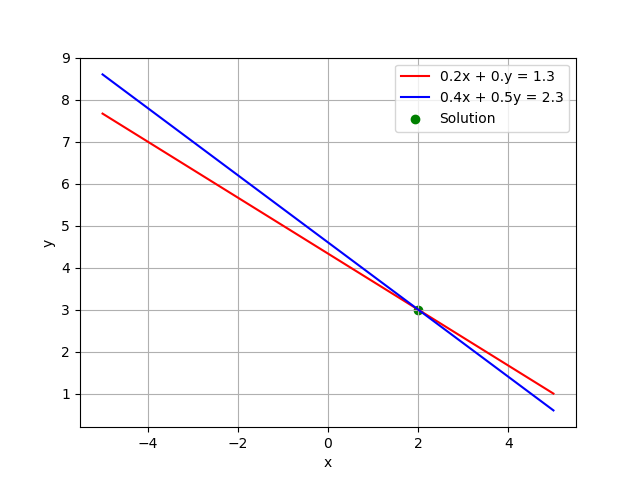
\includegraphics[width=1\columnwidth]{plots/plot.png}
   \caption{Solving the system of equations, $0.2x + 0.3y = 1.3, 0.4x + 0.5y = 2.3$}
   \label{stemplot}
\end{figure}
\end{document}
